
\documentclass[12pt]{report}
\usepackage[a4paper]{geometry}
\usepackage[myheadings]{fullpage}
\usepackage{amsmath}
\usepackage{fancyhdr}
\usepackage{lastpage}
\usepackage{graphicx, wrapfig, subcaption, setspace, booktabs}
\usepackage[T1]{fontenc}
\usepackage[font=small, labelfont=bf]{caption}
\usepackage{fourier}
\usepackage[protrusion=true, expansion=true]{microtype}
\usepackage[english]{babel}
\usepackage{sectsty}
\usepackage{url, lipsum}
\usepackage{siunitx}
\usepackage[space]{grffile}
\usepackage{amsfonts}
\sisetup{range-phrase = --, range-units = single}
\DeclareSIUnit\dBm{dBm}

\newcommand{\HRule}[1]{\rule{\linewidth}{#1}}
\newcommand{\figureinset}[3]{\llap{\parbox[b]{#2in}{#1\\\rule{0ex}{#3in}}}}

\newcommand*\chem[1]{\ensuremath{\mathrm{#1}}}
% This command adds optionality of units at right side of equation
\makeatletter
\providecommand\add@text{}
\newcommand\tagaddtext[1]{%
  \gdef\add@text{#1\gdef\add@text{}}}%
\renewcommand\tagform@[1]{%
  \maketag@@@{\llap{\add@text\quad}(\ignorespaces#1\unskip\@@italiccorr)}%
}
\makeatother


% \onehalfspacing
\setcounter{secnumdepth}{5}
\setcounter{tocdepth}{5}

%-------------------------------------------------------------------------------
% HEADER & FOOTER
%-------------------------------------------------------------------------------
\pagestyle{fancy}
\fancyhf{}
\setlength\headheight{15pt}
\fancyhead[L]{Serwan Asaad}
\fancyhead[R]{Delft University of Technology}
\fancyfoot[R]{Page \thepage\ of \pageref{LastPage}}
%-------------------------------------------------------------------------------
% TITLE PAGE
%-------------------------------------------------------------------------------

\begin{document}

\begin{titlepage}
\begin{center}
~\\ [4.0cm]
\textsc{\LARGE Delft University of Technology}
\\ [3.0cm]
\textsc{\Large Master Thesis}
\HRule{0.5pt} \\
\LARGE \textbf{\uppercase{Three month report}}
\HRule{2pt} \\ [0.5cm]

% Author and supervisor
\noindent
\begin{minipage}{0.4\textwidth}
\begin{flushleft} \large
\emph{Author:}\\
Serwan Asaad
\end{flushleft}
\end{minipage}%
\begin{minipage}{0.4\textwidth}
\begin{flushright} \large
\emph{Supervisor:} \\
Dr.~Alessandro Bruno
\end{flushright}
\end{minipage}
\\ [3.0cm]
{\large \today}
\end{center}

\end{titlepage}


\author{
        Serwan Asaad
        Student ID: 4323475 \\
        Delft University of Technology \\
        Kavli Institute of Nanoschience\\
        Quantum Nanoscience Department\\
        Quantum Transport Group\\
        DiCarlo Lab}

\tableofcontents
\newpage

%-------------------------------------------------------------------------------
% Section title formatting
\sectionfont{\scshape}
%-------------------------------------------------------------------------------

%-------------------------------------------------------------------------------
% BODY
%-------------------------------------------------------------------------------

\section*{Introduction}

The subject of my Master's thesis will be on ways of improving T1 and T2 coherence times for qubits. The past few months I have been learning about superconducting circuit quantum electrodynamics. I have learned what set-ups are used for performing measurements on cQED samples, and about the types of measurements that are performed.

Traditionally the measurements were performed using Labview software. However, in the months that I have been working in the DiCarlo lab, a transition in measurement software has taken place from Labview to the Python-based QTLab. I have been very involved in this transition, as an important part of my research will be to characterize a sample quickly and accurately. This will enable a fast cycle from sample fabrication to characterization, hopefully leading to rapid progress in the development of quantum computing using cQED.

The past few weeks the focus of my measurements has shifted towards the characterization of resonators. This is largely due to the fact that two of my colleagues, Alessandro Bruno and Gijs de Lange, are working on a paper on ways of improving the quality factor of resonators. A large part of the data was already obtained before I joined the group, but a last set of measurements was required using the dilution refrigerator I most often operate at. The reason is that its base temperature is at \SI{15}{\milli \kelvin}, which is considerably lower than the base temperature of the refrigerator at which the other measurements were performed, namely \SI{250}{\milli \kelvin}. Because my focus so far has been more on resonators than on qubits, the main topic of this report will be on resonators, and I will include the topic of qubits in my final thesis.

Because the relevant regime where resonators interact with qubits is the single-photon regime, a very weak signal must must be applied to determine its properties in that regime. At this point noise becomes a relevant issue. I will therefore also devote a section of this report on the subject of noise.

\newpage










\chapter{Resonators}
\label{chapter:Resonators}
% TODO:
% Mention that a resonator can be seen as an LC-circuit

Possible additional topics:
\begin{itemize}
    \item Material (Silicon, sapphire)
    \item Superconducting material NbTiN. Advantage is that
    \item Asymmetry (can refer to \cite[p.~192]{Geerlings})
    \item Lorentzian shape
\end{itemize}


When a signal enters a fridge it is attenuated in several stages and eventually enters the sample being measured. In the sample the signal travels through a feedline. One or more resonators can then be capacitively coupled to the feedline. Qubits can then also be capacitively coupled to the resonators, and a resonator can even be used to connect qubits, a so-called 'bus'. However in this report only discuss the resonators connected to a central feedline will be discussed.









\section{Coplanar waveguide}
% Todo:
% Talk a little about why the geometry of a coplanar waveguide is the way it is

\begin{wrapfigure}{r}{0.4\textwidth}
    \begin{center}
        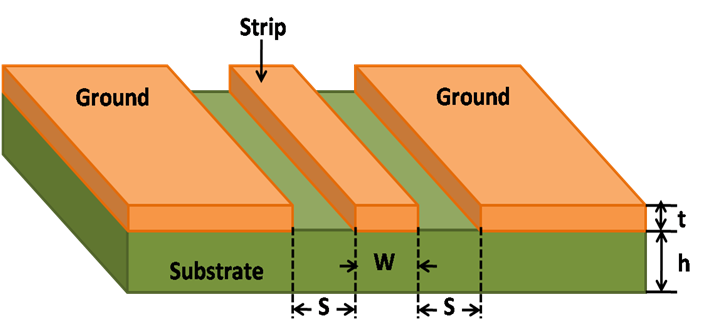
\includegraphics[width=.4\textwidth]{Figures/CPW.png}
    \end{center}
    \caption{Schematic of a coplanar waveguide.}
    \label{fig:CPW}
\end{wrapfigure}

In the context of circuit QED, one of the most common types of resonators are coplanar waveguides (CPW). Coplanar waveguides consist of a long central conducting track, with on both sides a neighbouring grounded track. The conducting track is seperated from the grounded tracks by a fixed distance.

One end is usually capacitively coupled to a feedline and has an open end, while the other end can either be open or shorted. This determines whether the resonant frequencies have a node or an antinode at that end. In the case of a shorted end, the resonant frequencies have an antinode at that end, resulting in a  $1/4 - \lambda$ resonator. This means that the wavelength fundamental mode fits $1/4$ times into the resonator. In the case of an open end, the resonant frequencies have an node at that end, resulting in a $1/2 \lambda$ resonator.









\section{Quality factor}
\label{sec:Quality factor}
% TODO
% Find where it says that loss tangents can be added to each other
% Include the fact that participation ratios are needed for adding quality factors of loss channels
% Explain why one wants a quality factor that is as high as possible
% Find place for equation FWHM
One important property of a resonator is its quality factor. Generally speaking, the quality factor of a resonator determines the ratio between energy stored in a resonator and the energy leaking away from the resonator. For cQED resonators this corresponds to the rate at which photons dissipate from the resonator. A high quality factor corresponds to a low dissipation rate.

The quality factor can also be defined as \cite[p.~23]{Mazin}:

\begin{equation}
    Q = \omega_0 \tau_1
\end{equation}
Here $\omega_0$ is the resonance frequency of the resonator, and $\tau_1$ is the decay time of the resonator. The decay time is the time taken by a resonator to dissipate its energy to $1/e$ of its original energy. One can see that this definition is in accordance with the first definition, as the energy is related to frequency through the Planck-Einstein relation: $E = \hbar \nu$, and therefore increases with increasing frequency.

\begin{equation}
    Q = \omega_0 / \Delta \omega
    \label{eq:FWHM}
\end{equation}

Photons can dissipate from the resonator through its different loss channels. Each of these loss channels has a corresponding quality factor. One such loss channel is due to resonators in cQED being capacitively coupled to a feedline. The quality factor associated to this loss channel is known as the coupling quality factor $Q_c$. This coupling quality factor depends on the amount of capacitive coupling between the resonator and the feedline. It can therefore be engineered to have a certain value, depending on the amount of interaction wanted between resonator and feedline.

The other loss channels are usually unwanted, and therefore desired to be as low as possible. These individual channels are usually lumped together, resulting in a combined quality factor, known as the intrinsic quality factor $Q_i$.

The total quality factor of the resonator is known as the loaded quality factor $Q_l$. It is related to $Q_c$ and $Q_i$ through:

\begin{equation}
    \frac{1}{Q_l} = \frac{1}{Q_c} + \frac{1}{Q_i}
    \label{eq:Q_l}
\end{equation}

From equation \ref{eq:Q_l} it can be seen that if the difference between $Q_c$ and $Q_i$ is large, then the loaded quality factor $Q_l$ will be approximately equal to the minimum of the two.


For a $1/4 - \lambda$ resonator the amplitude of transmission has a minimum $S_{21}^{min}$, given by \cite[p.~29]{Mazin}:
\begin{equation}
    S_{21}^{min} = \frac{Q_c}{Q_c + Q_i}
    \label{eq:S21min}
\end{equation}

With knowledge of the resonant frequency $\omega_0$, the resonant width $\Delta \omega$, and the transmitted signal at resonance $S_{21}^{min}$, it is possible through equations \ref{eq:FWHM} and \ref{eq:S21min} to determine both the coupling quality facto $Q_c$ and the intrinsic quality factor $Q_i$. Note that as equation~\ref{eq:S21min} depends on the ratio of the two quality factors,to get an accurate estimate of both quality factors, they should have a comparable value.

\begin{itemize}
    \item tan delta: loss channels, sum?
    \item Photon number dependence
    \item nonlinear effects (can refer to \cite{abdo2006nonlinear})
\end{itemize}





\section{Losses}

When a resonator is being driven at its resonance frequency, it is absorbing photons from the external source. When this external driving stops, the resonator slowly loses its photons through its different loss channels.

One loss channel was already discussed in section~\ref{sec:Quality factor}, namely through the coupling to the feedline. This loss channel is not unwanted, as the amount of coupling to the feedline determines how fast the resonator and feedline can interact with each other. The other loss channels, however, are unwanted. They cause dissipation of information. Some of the main causes of loss will be discussed in this section.


\subsection{Causes of loss}

\subsubsection{Two-level systems}
\label{sec:TLS}
% TODO mention that dissipation rate depends on electric field strength

Two-level systems (TLS) are systems which can be in a ground state or an excited state. In some cases they can be useful. In fact a qubit itself is an example of a TLS. In other cases, however, TLS can also be a source of dissipation. Study suggests that in cQED, most TLS reside in a thin oxide layer at the metal-substrate interface and the substrate-air interface \cite{wenner2011surface}.

Resonators are surrounded by a large quantity of TLS, each of which has its own resonance frequency, depending on its energy landscape. When the resonance frequency of a TLS is close to that of the resonator, it can absorb a photon from the resonator, upon which it tunnels to an excited meta-stable state. TLS have a finite lifetime in their excited state, after which they decay back to their ground state.

In the low power, low temperature regime, TLS reside mostly in their ground state, and only occasionally tunnel to the excited state, upon absorption of a photon. It is theorized that, in this regime, TLS are the main source of dissipation for resonators \cite{gao2008experimental}. At higher powers and/or temperatures, TLS will tunnel to an excited state at a higher rate. Due to their finite lifetime they become saturated at a certain point. Since the quality factor depends on the ratio between energy stored and energy dissipated, when the TLS are saturated the amount of dissipation is limited, while the energy stored can still increase. Therefore, in the low power, low temperature regime, increasing either of the two parameters results in an increase in quality factor. At a certain point, however, further increasing either of the two will not improve the quality factor. This is due to other effects dominating in these regimes.

\begin{itemize}
    \item To our knowledge, dielectric loss at low temperature
        arises from the presence of two-level states (TLS) formed
        by random bonds that tunnel between two sites. \cite{martinis2014ucsb}
    \item Mostly reside at surface \cite{gao2008experimental}
    \item 1/f noise \cite{burnett2013evidence}
    \item Dielectric materials (Table \cite{martinis2014ucsb})
\end{itemize}



\subsubsection{Quasiparticles}

Another source of dissipation for resonators is due to quasiparticles being present in the superconducting layer. When a Cooper-pair is broken up, Bogoliubov quasiparticles are formed \cite[p.~16]{Barends}. These quasiparticles can have either electron-like or hole-like properties. They are a source of dissipation for resonators, since they are non-superconducting and therefore cause the surface impedance to be slightly resistive \cite[p.~18]{Mazin}.

The breaking up of Cooper-pairs is due to excitations. These excitations can either be thermal, or due to photon absorption. Therefore an increase in temperature or an increase in photon density will result in a higher density of quasiparticles.

\begin{itemize}
    \item Quasiparticle excitation energy $E = \xi^2 + \Delta ^2$,
        where $\xi$ is the energy of the single particle in the normal state relative to the Fermi energy \cite{Barends}
    \item Increases with increasing frequency
    \item Decreases exponentially as the temperature decreases \cite[p.~19?]{Mazin}
    \item Quasiparticles are created through thermal excitation, but can also be excited by photons with $h \nu > 2 \Delta$\cite{Gao}
    \item Quasiparticles change the surface impedance of resonators, which can be measured.
        This technique is used to create MKID detectors \cite{Gao}
    \item "[Surface impedance] change is caused by quasiparticles blocking
        the Cooper pairs from occupying some of the electron states (through the exclusion principle), which
        modifies the effective pairing energy and reduces the density of pairs."\cite[p.~3]{Mazin}
    \item A lot of information in thesis by Lutchyn \cite{Lutchyn}
\end{itemize}




\subsubsection{Radiation}

A third source of dissipation is due to radiation from the resonator. This radiation is due to the spontaneous emission of photons.

The amount of dissipation due to radition is directly related through \cite{sage2011study,Mazin}:

\begin{equation}
    Q_{rad} = \alpha \left( \frac{L}{s + w}\right)^{n_r}
    \label{Qrad}
\end{equation}

As shown in Figure~\ref{fig:CPW}, $s$ is the distance between the conducting and grounded track, $w$ is the width of the conducting track. The parameter $\alpha$ depends on properties such as impedance and the dielectric constant of the substrate. From Formula \ref{Qrad} it is clear that a decrease of the conducting track width or the distance between tracks leads to an increase in $Q_{rad}$. However, with a decrease of either of the two parameters, the field strength close to the resonator becomes higher. If the TLS are not saturated (i.e. low power and temperature), this will increase the amount of dissipation through TLS. Therefore it is not necessarily advantageous to minimize $s$ and $w$.

Radiation loss becomes the dominant source of dissipation at high powers and/or temperatures, but otherwise usually is not the limiting factor. Since measurements relevant for quantum computing are usually operated at low power and temperature, this source of dissipation is usually less important than other sources, such as TLS dissipation.

\begin{itemize}
    \item Possible other useful sources: \cite{denlinger1969radiation} \cite{khalil2011loss}
\end{itemize}



\subsubsection{Vortices}


\begin{itemize}
    \item Trapped vortices cause parts to be non-superconducting
    \item Combatting trapped vortices with grid-like structure
\end{itemize}



\subsection{Minimizing losses}

\subsubsection{Surface treatment}

Previous research has determined that for resonators, TLS are mostly present at the surfaces \cite{gao2008experimental}. These oxides may reside at the interface between metal and dielectric, or between the dielectric and vacuum, or possibly between metal and vacuum (depending on the type of metal used). One explanation for TLS being present is the presence of an amorphous oxide layer at the interfaces. These oxides may act as TLS. During deposition of the metal on the dielectric, this oxide layer can become trapped between the two interfaces. For a silicon dielectric, this oxide layer can be removed by shortly treating the sample with hydrophluoric acid. This process is also known as an 'HF dip'.

Aside from the HF dip, additional surface treatment can be applied. For the resonators measured in this report, before depositing the metal on the substrate, an additional exposure to hexamethyldisilazane (HMDS) was applied. The reason for this additional step is that there is a lattice mismatch between the metal and substrate. The intermediate layer of HMDS can possibly mediate this lattice mismatch. See \cite{DRIE} for more information.


\subsubsection{Infrared shielding}

Aside from thermal excitation, quasiparticles are also formed from the absorption of photons. High-frequency photons (UV-range or higher) are usually not a significant contribution, as they are easily absorbed by materials, well before they reach the inner layers of the fridge. Lower-frequency photons, such as in the infrared range, however, can penetrate through the fridge to the sample. These infrared photons can cause the excititation of quasiparticles. By using infrared shielding, such as a coating film inside the fridge, the amount of infrared radiation reaching the sample can be lowered.



\subsubsection{Deep-reactive ion etching}

Another technique applied to the resonators studied in this report is deep-reactive ion etching (DRIE), which is a type of Bosch process \cite{DRIE}. In this technique two alternating steps are performed:

\begin{enumerate}
    \item An etching step in which an $\chem{SF_6}$ plasma is used to etch the substrate layer.
    \item A passivation step in which $\chem{C_4H_8}$ is released. The gas forms a protective layer on the substrate, except for the direction in which the etching plasma is accelerated. The result is that the sidewalls are protected from the etching process
\end{enumerate}

Using DRIE, nearly vertical sidewalls can be created for the substrate. The result is that the substate-air interface is removed from the regions between the CPW tracks, which are the regions where the electric field strength is high. As the dissipation due to TLS depends on the electric field strength, it is expected that DRIE will result in a lower TLS dissipation rate at this interface.



\section{Experimental set-up}


\begin{wrapfigure}{r}{0.4\textwidth}
    \begin{center}
        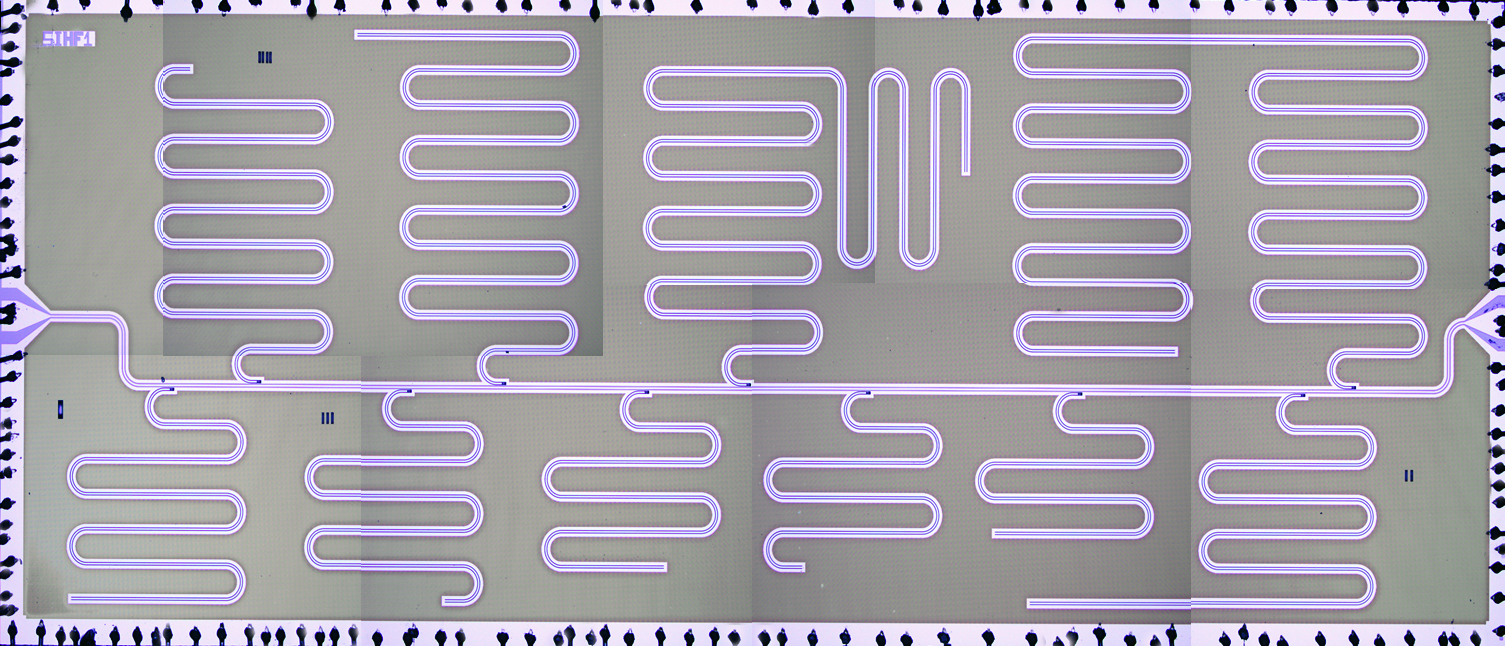
\includegraphics[width = .4\textwidth]{Figures/All_set4.png}
    \end{center}
    \caption{Optical microscopy image of the sample measured in this report. The sample consists of ten $1/4 - \lambda$ resonators, with frequencies ranging between \SIrange{1}{11}{\giga \hertz}, connected to a central feedline. The resonators are made using NbTiN on a Si substrate. The sample is treated with HMDS and DRIE.}
    \label{fig:set4}
\end{wrapfigure}

The fridge used in this experiment is a dilution refrigerator, made by Leiden Cryogenics. The refrigerator has a base temperature of \SI{\sim15}{\milli \kelvin}. An input signal was generated using a Rohde \& Schwarz ZVM vector network analyzer, connected to an Aeroflex 8310 step attenuator, which has an attenuation range of \SI{120}{\decibel}. The signal out of the fridge was measured using the same vector network analyzer.

Using this set-up $1/4 - \lambda$ resonators, fabricated by Alessandro Bruno, were measured in a frequency range between \SIrange{1}{9}{\giga \hertz}. The sample is shown in Figure~\ref{fig:set4}. The resonators were made using NbTiN on a silicon substrate. The advantage of NbTiN is that the metal atoms are bound to nitrogen, thereby inhibiting bond formation with oxides. In a way to minimize losses, all resonators were treated with HMDS and deep-reactive ion etching.

By driving a signal through the feedline, the resulting transmitted signal $S_{21}$ can be measured. At or close to the resonance frequency of a resonator, the resonator will either cause enhanced transmission ($1/2 \lambda$ resonator), or diminished transmission ($1/4 \lambda$ resonator).

Unless stated otherwise, all measurements were performed with the fridge at base temperature (\SI{\sim15}{\milli \kelvin}).

\section{Results and discussion}


\subsection{Resonator measurement}

\begin{figure}[h]
    \centering
    \begin{subfigure}[b]{.49\textwidth}
        \label{fig:resonator_amplitude}
        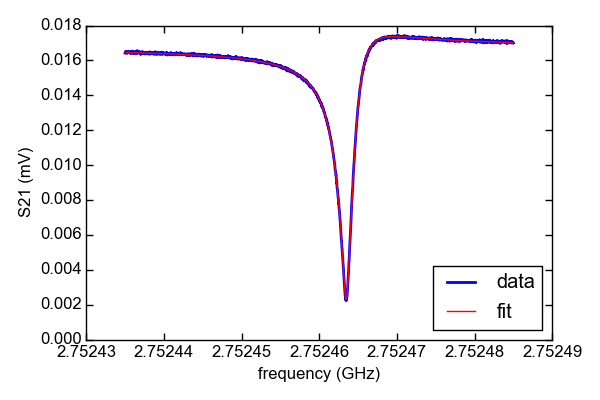
\includegraphics[width=\textwidth]{Figures/resonator_amplitude.png}\figureinset{(a)}{2.55}{2.0}
    \end{subfigure}
    \begin{subfigure}[b]{.49\textwidth}
        \label{fig:resonator_complex}
        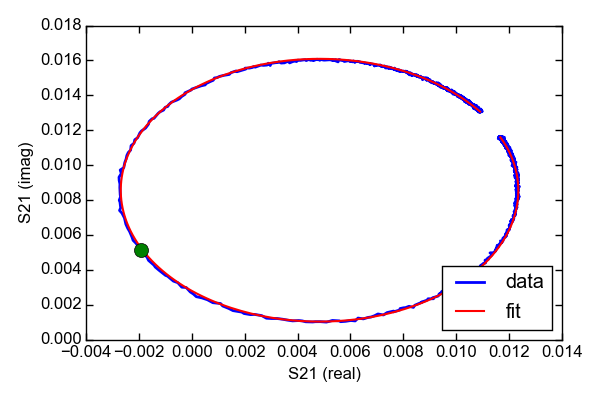
\includegraphics[width=\textwidth]{Figures/resonator_complex.png}\figureinset{(b)}{2.55}{2.0}
    \end{subfigure}
    \caption{Forward transmission $S_{21}$ spectrum of a resonator around \SI{2.75}{\giga \hertz}. Panel (a) shows the amplitude of $S_{21}$, along with a fit (red). Panel (b) shows the path of $S_{21}$ in the complex path, along with a fit (red). The green dot indicates the resonance frequency of the resonator.  Measurement was performed at \SI{15}{\milli \kelvin} at an input power of \SI{-123}{\dBm} corresponding to $\sim 5 \times 10^4$ photons.}
    \label{fig:resonator}
\end{figure}

 In Figure~\ref{fig:resonator} the transmission $S_{21}$ of a resonator is shown. Figure~\ref{fig:resonator_amplitude} shows the transmitted voltage $|S_{21}|$ of the resonator as a function of frequency. As one can see, the resonator has a shape similar to a Lorentzian dip. One interesting point is that the Lorentzian exhibits an asymmetry, which is often attributed to reflections in the feedline \cite[p.~192]{Geerlings}. This could be caused by impedance mismatching.

 % TODO
 % Say something about complex data

\subsection{Power dependence}
\label{sec:resonator:results:power_dependence}

\begin{figure}
    \centering
    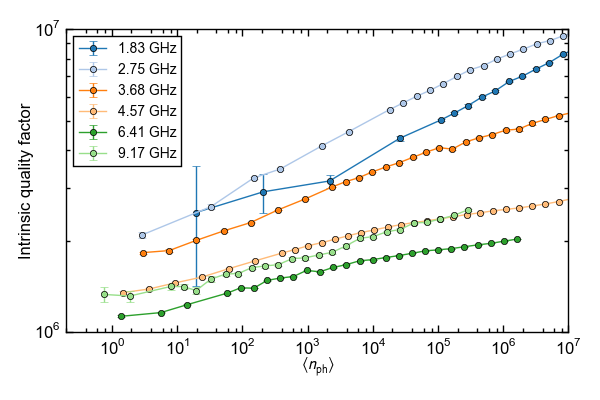
\includegraphics[width=0.8\textwidth]{Figures/Qi_vs_n_photon.png}
    \caption{Intrinsic quality factor of resonators as a function of mean number of photons present in the resonator. Measurements were performed at \SI{15}{\milli \kelvin}.}
    \label{fig:Qi_vs_n_photon}
\end{figure}
To be able to study the behaviour of the resonators, measurements were performed for several powers. Using proper calibrations for the attenuation down to the sample, the power can be converted to the input power at the sample. This value can then be converted to the mean number of photons present in the resonator \cite{DRIE}. The results are shown in Figure~\ref{fig:Qi_vs_n_photon}.

As can be seen, the internal quality factor $Q_i$ of all resonators decrease with decreasing photon number. One explanation for this phenomenon is that the dissipation dissipation is mainly due to TLS. Since measurements were performed at \SI{\sim15}{mK}, the TLS are not saturated since the rate of thermal excitation is low. As discussed in section~\ref{sec:TLS}, the loss due to TLS is highest at low power, in the regime where they are not saturated. Therefore the fact that the internal quality factor $Q_i$ rises with the mean number of photons present in the resonator can be attributed to a larger amount of TLS being satured. This would suggest that, even with HMDS and DRIE treatment of the sample, the internal quality factor is still limited by TLS being present.

The mean photon number of a resonator is inversely proportional to the square of frequency \cite{DRIE}, so for resonators with a low frequency a lower input power is required than with a high frequency. At high photon numbers this is not a concern, as the transmitted signal is high enough to be accurately measured in a short period of time. For the single-photon powers, however, which is the region of interest for quantum computation, acquiring enough signal took up to five hours for the lowest frequencies. The reason that for the resonator with a resonance frequency at \SI{1.83}{\giga \hertz} has large error bars at low powers can be partly attributed to this, but as we will see in section \ref{sec:noise_results}, the main reason is that its frequency lies outside the bandwidth of the amplifiers and circulators of the set-up.

\begin{itemize}
    \item Quality factor depends on frequency?
    \item One can also see that the quality factor is lower for resonators with higher resonance frequency.
\end{itemize}




\subsection{Temperature dependence}
\label{sec:resonator:results:emperature_dependence}
\begin{figure}
    \centering
    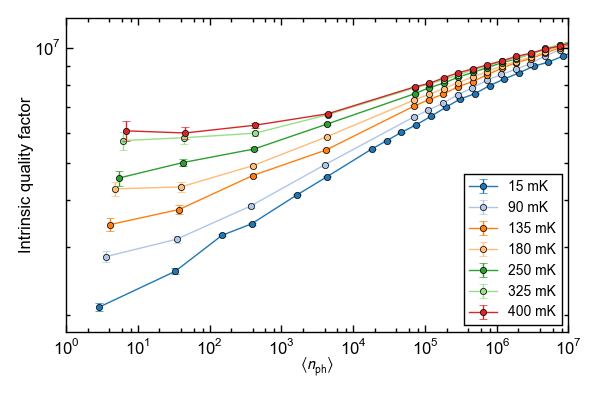
\includegraphics[width=0.8\textwidth]{Figures/Qi_vs_n_photon_temperature_dependence.png}
    \caption{Intrinsic quality factor versus photon number for temperatures ranging from \SI{15}{\milli \kelvin} up to \SI{400}{\milli \kelvin}. All measurements were performed for a resonator with resonance frequency $f_0 = $\SI{2.75}{\giga \hertz}.}
    \label{fig:Qi_vs_n_photon_temperature_dependence}
\end{figure}

Aside from power, some of the dissipation channels also depend on the temperature of the system. To be able to study the effect of temperature on resonators, the resonator with frequency \SI{2.75}{\giga \hertz} has been studied as a function of power for several temperatures ranging from \SI{15}{\milli \kelvin} up to \SI{400}{\milli \kelvin}. The reason for choosing this resonator is that it has the highest internal quality factor of all the resonators measured, and so any change in quality factor would be most clearly visible.

The results are shown in Figure~\ref{fig:Qi_vs_n_photon_temperature_dependence}. As can be clearly seen, the quality factor increases with increasing temperature. This is likely due to the fact that TLS are thermally excited for a larger percentage of time. Therefore, the relative energy dissipation with respect to total energy in the resonator will be lower, resulting in an increase in quality factor.

Another interesting point is that the increase in quality factor as a function of temperature is largest at low powers. This can also be explained when the limiting factor is due to TLS. With low powers, the TLS are almost exclusively excited thermally, while at higher powers, the excitation of TLS is not only due to thermal excitations, but also from photon absorption.

If one looks at the highest temperatures, it seems that the increase in quality factor as a function of temperature seems to slowly approach a saturation point. One reason is that the TLS are approaching their saturation, and so increasing the temperature further will have little effect on the percentage of time that the TLS are in the excited state. As will be shown in the next section, the quality factor is close to its maximum value, and will decrease as temperature is increased further.



\subsection{Temperature tracking}
\label{resonator:results:temperature_tracking}
% TODO
% Find out the name of the process that occurs at 1K.
% Make stronger statement supporting claim that quasiparticles are dominant source at higher temperatures
% Maybe also mention the rapid shift of resonator frequency during beginning stage of cooldown

\begin{figure}[h]
    \centering
    \begin{subfigure}[b]{.49\textwidth}
        \label{fig:temperature_tracking_Qi_drop}
        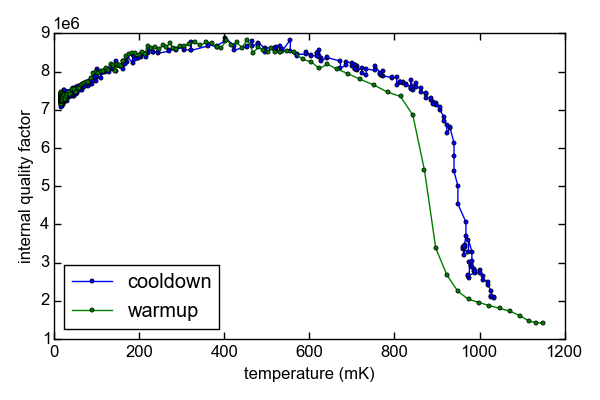
\includegraphics[width=\textwidth]{Figures/Temperature tracking drop - Qi vs T.png}\figureinset{(a)}{2.65}{1.92}
    \end{subfigure}
    \begin{subfigure}[b]{.49\textwidth}
        \label{fig:temperature_tracking_Qi_nodrop}
        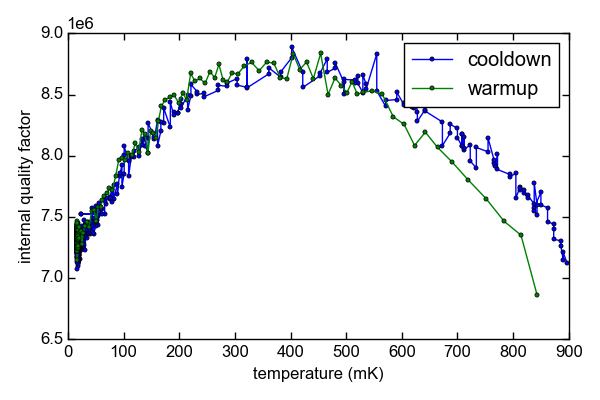
\includegraphics[width=\textwidth]{Figures/Temperature tracking - no drop - Qi vs T.png}\figureinset{(b)}{2.57}{1.92}
    \end{subfigure}
    \caption{Internal quality factor versus temperature for the resonator with resonance frequency $f_0= $\SI{2.75}{\giga \hertz}. Quality factor was continuously measured as the sample was cooled down and warmed up four days later. Panel (a) shows the full temperature range up to the helium condensation cycle. Panel (b) shows a close-up of the region until \SI{900}{\milli \kelvin}.}
    \label{fig:temperature_tracking_Qi}
\end{figure}
`'
To further investigate the temperature dependence of the resonator, a continous measurement was performed on the resonator with resonance frequency \SI{2.75}{\giga \hertz} during a cool-down and a subsequent warm-up of the fridge four days later. Measurements were performed for temperatures ranging from base temperature (\SI{15}{\milli \kelvin}) to roughly \SI{1}{\kelvin}. Above this temperature, the fridge entered a cyclic ... TODO. All temperatures were measured at an input power of \SI{-113}{\dBm}, corresponding to roughly $5 \times 10^5$ photons. In Figure \ref{fig:temperature_tracking_Qi} the internal quality factor versus temperature is shown during a cooldown and subsequent warm-up of the fridge. As can be seen, the quality factor reaches a maximum quality factor at a temperature of \SI{\sim600}{\milli \kelvin}. Below this temperature, the quality factor is likely limited by the presence of TLS (see sections \ref{sec:resonator:results:power_dependence} and \ref{sec:resonator:results:emperature_dependence}). Above this temperature however, the quality factor decreases, indicating that TLS are not the limiting factor anymore for $Q_i$. One possibility is that the main source of dissipation is now due to the presence of quasiparticles in the resonator. At even higher powers other effects, such as vortices and enhanced radiation, contribute more and more significantly to the decay of the quality factor.

From Figure~\ref{fig:temperature_tracking_Qi} it seems that there is some hysteresis at high temperatures. This is likely due to the fact that the thermometer is at a different position in the fridge as the sample, and does not thermalize equally fast. There may therefore be a delay between the temperature of the thermometer, and the actual temperature of the sample.

% ADD figure of resonance frequency

\begin{figure}[h]
    \centering
    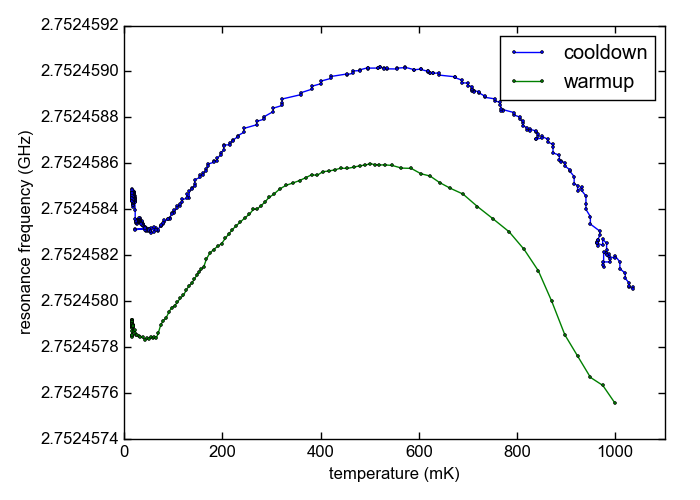
\includegraphics[width=.7\textwidth]{Figures/Temperature tracking - f0 vs T.png}
    \caption{Resonance frequency versus temperature during a cooldown and subsequent warm-up four days later. In the period between cooldown and warm-up the resonance frequency has shifted by \SI{\sim 500}{\hertz}, possibly due to phase noise.}
    \label{fig:temperature_tracking_f0}
\end{figure}


Aside from the internal quality factor, another quantity of interest is the resonance frequency $f_0$ of the resonator, which also depends on the temperature. The result from of tracking the resonance frequency of the resonator during cooldown and subsequent warm-up is shown in Figure~\ref{fig:temperature_tracking_f0}. As can be seen in both cases, the resonance frequency reaches a maximum around \SI{500}{\kelvin}.

B
e++++++++++tween the cooldown and warm-up the resonance frequency seems to have shifted by roughly \SI{500}{Hz}. As the sample was kept at \SI{15}{\milli \kelvin}, it is unlikely that this decrease in resonance frequency is due to degradation of the sample. One possible explanation is that this change in resonance frequency is due to phase noise, which is known to shift the resonance frequency of the resonator. Further measurements are, however, required to determine if this is the case.

The decrease in resonance frequency at higher temperatures can be explained by the presence of quasiparticles, which increase the kinetic inductance \cite[p.~91]{Geerlings}. The resonance frequency is inversely proportional to the square root of the total conductance \cite{barends2008contribution}, and so an increase in kinetic inductance leads to a decrease in resonance frequency. For measurements done by Barends et al. \cite{barends2008contribution}, the change in resonance frequency due to changes in the kinetic inductance seem to roughly correspond with the decrease in center frequency measured in Figure~\ref{fig:temperature_tracking_f0}.

\begin{figure}[h]
    \centering
    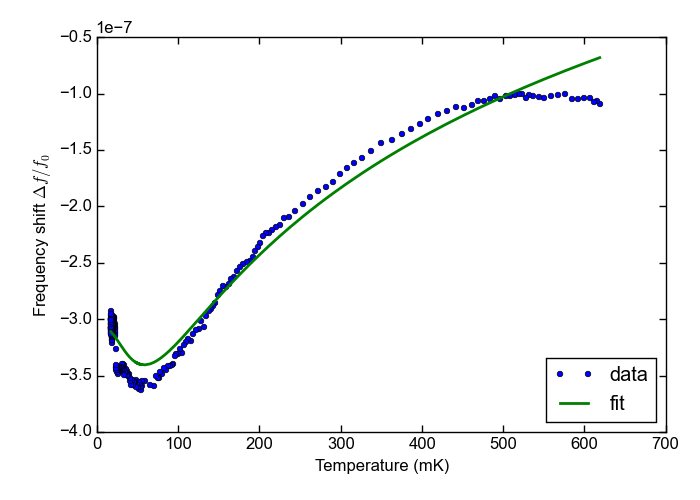
\includegraphics[width=.7\textwidth]{Figures/Temperature increase tracking - f0 vs T with fit.png}
    \caption{Frequency shift versus temperature for low temperatures, along with fit (green). The fit was performed using the model by Gao et al.~\cite{gao2008experimental}. The fit corresponds well with data, even describing the frequency peak at the lowest temperatures.}
    \label{fig:f0_vs_T_with_fit}
\end{figure}

The decrease in resonance frequency at lower temperatures can be explained due to still being present. A model is presented by Gao et al. \cite{gao2008experimental}, in which they describe the decrease in resonance frequency due to the presence of TLS. As can be seen in Figure~\ref{fig:f0_vs_T_with_fit} the model corresponds well with the data at low temperatures. At higher temperatures the model deviates from data, which may be explained by quasiparticles dominating as source of dissipation. An interesting thing to note is that an increase in resonance frequency was predicted at the lowest temperatures, but as they did not reach temperatures sufficiently low they could not confirm this effect. In Figure~\ref{fig:f0_vs_T_with_fit} however, this increase in resonance frequency is observed. This supports the claim that at low temperatures the resonator is still limited by TLS, even after treatment of HMDS and DRIE.

\begin{itemize}
    \item Info at Geerlings \cite[p.~106]{Geerlings}. Seems to say that resonance frequency depends on kinetic inductance, but also on TLS
    \item Mention that resonance frequency also depends on TLS
    \item At higher temperatures kinetic inductance takes over: \cite{barends2008contribution}, \cite[ch.~3]{Gao}
\end{itemize}



\section{Conclusion and future work}

Since the quality factor of all resonators is found to decrease with decreasing input power, this indicates that at low temperatures and powers the limiting factor is still due to TLS. The fact that the quality factor initially increases with higher temperatures, supports this claim. By also measuring  the resonance frequency as a function of temperature, the curve obtained is in good agreement with a model describing the resonance frequency shift due to TLS \cite{gao2008experimental}. The curve even shows an increase in resonance frequency at the lowest temperatures, which was also predicted by the model. These results suggest that even after HMDS surface treatment and deep-reactive ion etching was applied, the internal quality factor of the resonator at low temperatures and power is still limited by the presence of TLS.

Nevertheless, As shown by Bruno et al. \cite{DRIE}, the application of HMDS surface treatment and DRIE resulted in an improvement of the internal quality factor of the resonators by almost an order of magnitude. More research must be done to determine at what interface the dissipation due to TLS is greatest after these two treatments.

The next step is to perform the same treatments (HMDS and DRIE) on transmon qubits, to study what the influence will be on coherence times.



% \chapter{Measurements}



% \section{Heterodyne detection}
% \begin{itemize}
%     \item Idea to also obtain complex signal
% \end{itemize}

% \section{Vector network analyzer}
% \begin{itemize}
%     \item Complex signal
% \end{itemize}

% \section{Conclusion and future work}

% \begin{itemize}
%     \item One goal is to set-up the complex signal heterodyne system and compare it to the Vector network analyzer
% \end{itemize}













\newcommand{\vrms}{\text{v}_\text{n}^\text{rms}}
\newcommand{\vsq}{\overline{\text{v}_\text{n}^2}}
\newcommand{\vn}{\text{v}_\text{n}}
\newcommand{\vin}{\text{v}_\text{in}}
\newcommand{\vout}{\text{v}_\text{out}}
\newcommand{\Sin}{\text{S}_{\vn}^\text{in}}
\newcommand{\Sout}{\text{S}_{\vn}^\text{out}}
\newcommand{\Svn}{\text{S}_{\vn}}




\chapter{Noise}
% TODO: p~256 of electric noise book (deals with amplifier circuits)

% TODO: Left to find out:
% Is the power to V_in conversion correct?

When performing measurements one is faced with the reality that no component is ideal. When a signal passes through the different parts of a set-up, noise is constantly being added. Noise is the term given for all the random fluctuations that are added to the signal. These fluctuations are the cumulative result of several noise source contributions.

Thermal noise is one of the most common sources of noise. It is the result of the random thermal fluctuations of electrons. It is an example of frequency-independent noise, also known as white noise. Noise sources can also be frequency-dependent, such as TLS, as discussed in Chapter~\ref{chapter:Resonators}. This is an example of $1/f$-noise: the amount of noise added increases with decreasing frequency. In fact, truly frequency-independent noise does not exist, as even white noise has been observed to decrease at extremely high frequencies (\SI{\sim e15}{\hertz}). At these frequencies a quantum correction needs to be added \cite[p.~50]{vasilescu2006electronic}.

When performing measurements one important question to ask is how much noise is being contributed to the signal. In this chapter a model is presented for the general set-up used for measuring superconducting resonators and qubits. Using this model it is possible to characterize the amount of noise by determining its associated noise temperature. Finally, this model is applied to the set-up used to characterize the resonators presented in Chapter~\ref{chapter:Resonators}.

\section{Characterizing noise}

\subsection{Circuit representations}


\begin{figure}[h]
    \centering
    \begin{subfigure}[b]{.43\textwidth}
        \includegraphics[width=\textwidth]{Figures/thevenin.png}%\figureinset{(a)}{2.55}{1.5}
        \caption{Th\'evenin representation}
        \label{fig:thevenin}
    \end{subfigure}
    \begin{subfigure}[b]{.49\textwidth}
        \includegraphics[width=\textwidth]{Figures/norton.png}%\figureinset{(b)}{2.55}{1.5}
        \caption{Norton representation}
        \label{fig:norton}
    \end{subfigure}
    \caption{Two equivalent representations of a system containing noise. Panel~\textbf{(a)} shows the Th\'evenin representation, in which a noiseless voltage source is connected in series with a noise voltage source. Panel~\textbf{(b)} shows the Norton representation, in which a noiseless current source is connected in parallel with a noise current source.}
\end{figure}

There are two circuit representations in which we can depict a system with a noise contribution: The Th\'evenin representation, and the Norton representation. In the Th\'evenin representation we can model the system as a voltage source, and the noise added to the system is a noise voltage source connected in series. In the Norton representation the system is a current source and the noise added is a noise current source connected in parallel to the current source. These two representations are identical and can be converted to each other. In this section we will adopt the Thev\'enin representation, and so the signal will be a voltage source combined in series with a noise voltage source.

Assuming the signal to be at a fixed frequency $\omega$ and amplitude $A$, the combined voltage $v(t)$ is then given by:

\begin{equation}
    \text{v}(t) = \text{v}_\text{signal}(t) + \text{v}_\text{noise}(t) = A \cos{\omega t} + \vn(t)
\end{equation}

The mean value of the noise voltage $\overline{\vn}$ is equal to zero. The amount of noise can be quantified by the root-mean square noise voltage $\vrms$:
\begin{equation}
    \vrms = \sqrt{\overline{\text{v}^2} - \overline{\text{v}}^2} = \sqrt{\vsq}
    \label{eqn:v_rms}
\end{equation}

\subsection{Noise power spectral density}

One way of quantifying the noise of the system is through the noise power spectral density $S(f)$, which is the distribution of noise per unit bandwidth as a function of frequency. For the Th\'evenin representation, the noise spectral density is defined in terms of voltage. When the only noise in the system is white noise, the spectral density is independent of frequency. It is then given by:

\begin{equation}
    S = \frac{\vsq}{\Delta f}
    \tagaddtext{[\si[per-mode=symbol]{\volt \squared \per \hertz}]}
    \label{eqn:noise spectral density definition}
\end{equation}

In this equation $\Delta f$ is the noise bandwidth. This is the bandwidth over which the noise is measured.

\newpage
\section{The model}

\begin{figure}
    \centering
    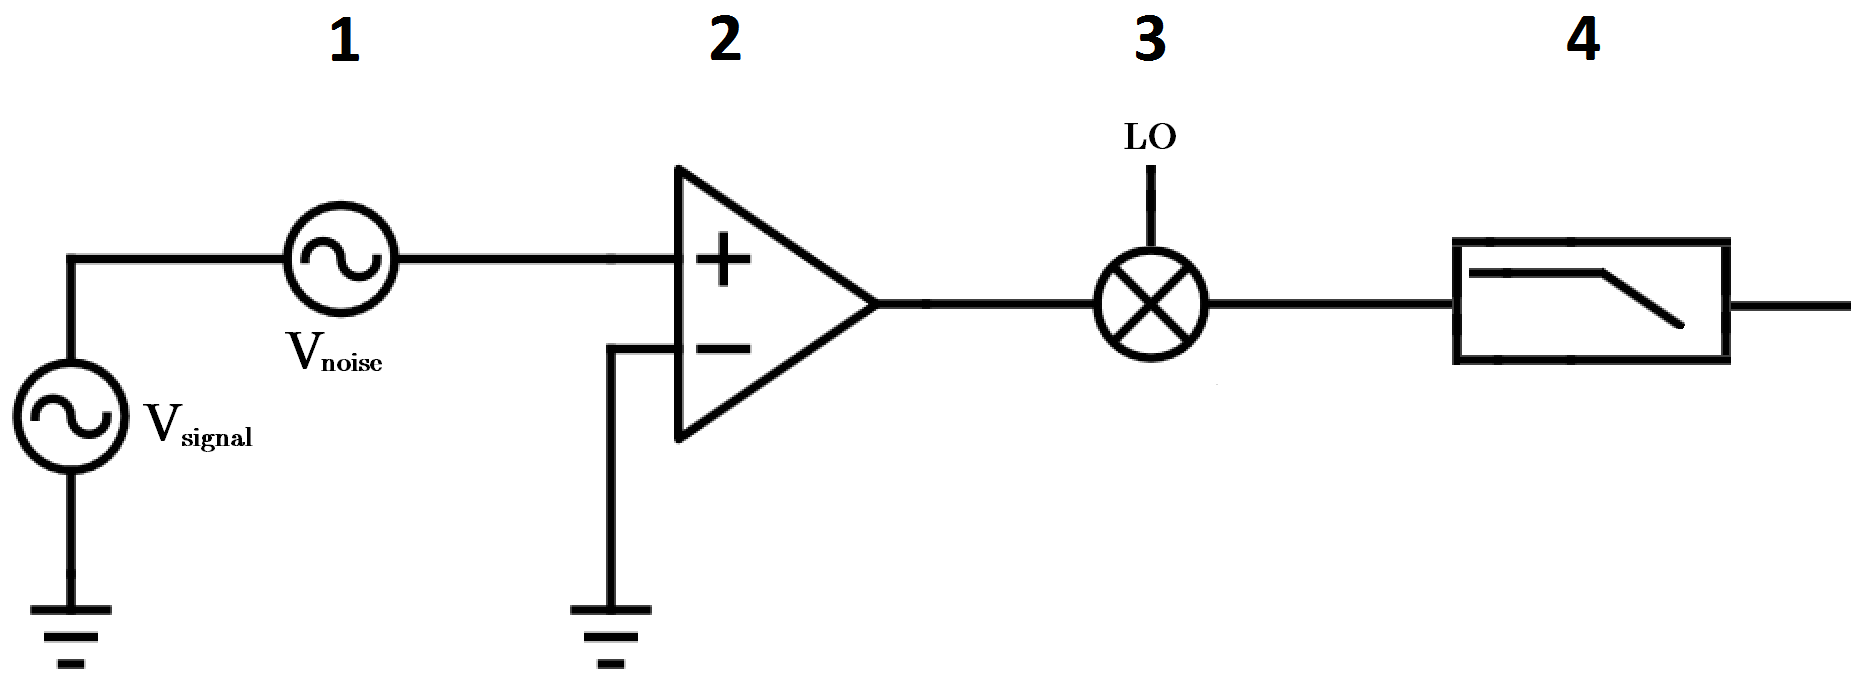
\includegraphics[width=.8\textwidth]{Figures/Noise model.png}
    \caption{Schematic representation of the measurement set-up including a noise source.}
    \label{fig:noise model}
\end{figure}


As shown in the schematic in Figure~\ref{fig:noise model}, we can model our set-up as a combination of four elements:

\begin{enumerate}
    \item A noise source.
    \item An amplifier to amplify the weak signal exiting the fridge.
    \item A mixer to downconvert the signal.
    \item A low-pass filter to remove unwanted high-frequency signal.
\end{enumerate}



\subsection{Noise source}

Using the Th\'evenin model, we can approximate the components up to the first amplifier in the fridge as a voltage source, with a noise voltage source connected in series.

We can include the noise added by the amplifier in the noise voltage source, in which case we assume the amplifier to be ideal. Furthermore, we assume the signal to be amplified sufficiently, such that the mixer and low-pass filter add a negligible amount of noise. We also ignore effect such as mixer leakage. With these assumptions all of the noise is originated from the noise voltage source.

We can associate an effective noise temperature to the noise voltage source. The noise temperature is defined as the temperature at which a resistor would produce an equal amount of noise. Note that, since we are comparing the system to a resistor, the noise needs to have an (approximately) white spectrum.

According to Nyquist's theorem \cite[p.~47]{vasilescu2006electronic}, if the system experiences white noise, and is in thermal equilibrium, the root-mean square noise voltage $\vrms$ is given by:

\begin{equation}
    \vrms = \sqrt{\vsq} = 4 k_B T R \Delta f
    \label{eqn:noise rms voltage}
\end{equation}

In this equation $\Delta f$ is the bandwidth over which the noise is integrated, $k_B$ is the Boltzmann constant, $T$ is the noise temperature of the noise source, and $R$ is the impedance of the system. We see that the noise added depends linearly on the bandwidth over which is integrated.

Combining Equations~\ref{eqn:noise spectral density definition} and \ref{eqn:noise rms voltage}, the noise power spectral density $S_{\vn}$ can be rewritten as:

\begin{equation}
S = \frac{\vsq}{\Delta f} = 4 k_B T R
\end{equation}





\subsection{Amplification}
During the amplification stage both the signal and the noise is amplified by the same amount. This amount of amplification is determined by the gain $G$, which is defined as the ratio between the output voltage and the input voltage:

\begin{equation}
    G = \frac{\text{v}_\text{out}}{\text{v}_\text{in}}
    \label{eqn:gain}
\end{equation}

According to the maximum power transfer theorem, the maximum power transfer between a source and load occurs when the impedances of source and load are matched, in which case half of the power is transferred. From this it follows that in the amplification process half of the signal is dissipated. However, as $G$ is defined as the ratio between $\text{v}_\text{out}$ and $\text{v}_\text{in}$ (Equation~\ref{eqn:gain}), the factor $\frac{1}{2}$ is included in $G$.

During amplification not only the signal is amplified with gain G: the noise is amplified by the same amount. Defining the noise power spectral density before amplification as $S^\text{in}$, and after amplification as $S^\text{out}$, the following relation holds:

\begin{equation}
    S^\text{out} = G^2\; S^\text{in} = G^2 4 k_B T R
    \label{eqn:noise power spectral density amplification}
\end{equation}

Note that the gain $G$ is squared, since the noise power spectral density depends quadratically on the root-mean square noise voltage. (TODO improve sentence)

In our actual set-up the amplification occurs in multiple stages. Aside from amplifying the signal and its noise, at each stage additional noise, originating from the amplifier itself, is added as well. This added noise is then also amplified in the next amplification stage.   Therefore it is always best to have the amplifier with highest gain and lowest noise temperature as the first amplifier in the chain. For more information see Friis formula \cite[p.~103]{vasilescu2006electronic}.



\subsection{Downconversion}

After amplification the frequency $\omega$ of the signal is still in the GHz range. In homodyne or heterodyne detection the signal is downconverted to DC (homodyne) or to a lower frequency (heterodyne), such that it can be measured more easily. To downconvert the signal, it is mixed in a mixer with a local oscillator (LO) signal having the same frequency $\omega$ (homodyne) or a slightly higher frequency $\omega + \Delta \omega$ (heterodyne). The mixer effectively multiplies the two signals (TODO: mention why amplitude of LO signal is unimportant). If the signal exiting the amplifier is given by $\text{v}(t) = A\cos \omega t$, then, ignoring a possible phase difference, the signal at the output of the mixer is given by:

\begin{align}
    \text{v}(t) \cdot \cos{\omega t}& = A \cos{\omega t} \cdot \cos{(\omega + \Delta \omega ) t} \notag\\
        & = \frac{1}{2} A \left[\cos{(2\omega + \Delta \omega)t} + \cos{\Delta \omega t}\right]
        \label{eqn:mixer}
\end{align}

As can be seen from Equation~\ref{eqn:mixer}, the output signal contains both the sum and the difference of the two signals. However, as the sum of both frequencies is in the GHz range, it can be filtered out using a low-pass filter, leaving only the downconverted signal, which is the result of the difference between the two frequencies. Note that the amplitude of the signal is reduced by a factor two. The noise amplitude is also reduced by a factor 2. Furthermore, in the case of a homodyne set-up, the difference signal is simply a DC signal ($\Delta \omega = 0$), while in the case of heterodyne the signal still contains a slow frequency $\Delta \omega$. For simplification we assume our set-up to be a homodyne set-up.

\subsection{Low-pass filtering}

In the case of homodyne detection the signal at the frequency of interest is downconverted to DC. However, the signal at other frequencies have not disappeared; in the mixer these have also shifted in frequency. Since the signal of interest is at DC, a low-pass filter can be used to filter out signal above a certain frequency.

The frequency above which a low-pass filter will filter out the signal is defined by its cut-off frequency $f_\text{c}$. The cut-off frequency $f_\text{c}$ is the frequency at which the signal is attenuated by \SI{3}{\decibel}. For first-order low-pass filters the noise bandwidth $\Delta f$ is related to the filter cut-off frequency $f_\text{c}$ by \cite[p.~81]{vasilescu2006electronic}:

\begin{equation}
    \Delta f = \frac{\pi}{2} f_\text{c}
    \label{eqn:noisebandwidth}
\end{equation}

\section{Noise temperature}

In the previous sections the influence of each of the components on the signal and on the noise has been analyzed. Using this information it is possible to determine the signal-to-noise ratio (SNR). The signal-to-noise ratio is the ratio between the average power of the signal and the average power of the noise, and is a measure for how well a signal can be separated from the noise.


\begin{align}
    \text{SNR} = \frac{\overline{\vout}^2}{\vsq} = & \frac{1/4 \;G^2 \; \overline{\vin}^2}{1/4 \; \Sout \; \Delta f}\notag\\
        = & \frac{G^2 \; \overline{\vin}^2}{G^2 \; \Sin \;\frac{\pi}{2}\;f_\text{c}}\notag\\
        = & \frac{\overline{\vin}^2}{2\;\pi \; k_B \; T \; R \; f_\text{c}}
    \label{eqn:SNR}
\end{align}

Note that the factors $1/4$ are due to the amplitude being lowered by a factor of $2$ due to mixing. Equation~\ref{eqn:SNR} can be rewritten such that we have an expression for the noise temperature of the system:

\begin{equation}
    T =\frac{\overline{\vin}^2}{2\; \pi \; k_B \; R \; f_\text{c} \; \text{SNR}}
    \label{eqn:noise temperature}
\end{equation}


\section{Results}
\label{sec:noise_results}
\begin{figure}[h]
    \centering
    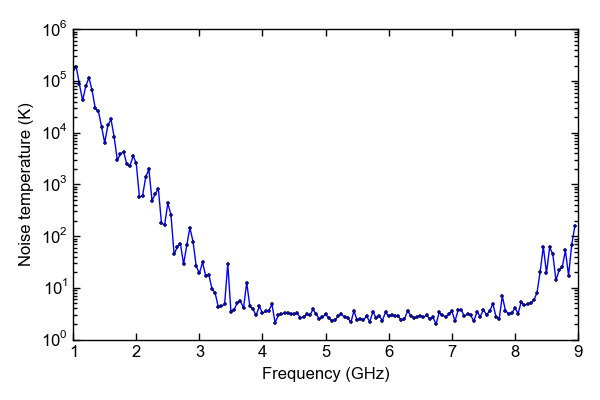
\includegraphics[width = .7 \linewidth]{Figures/noise_temperature_versus_power.png}
    \caption{Noise temperature versus frequency. The noise temperature has been calculated for $160$ frequencies in the range \SIrange{1}{9}{\giga \hertz}. For each frequency $2001$ points were measured, from which the signal, noise, SNR, and noise temperature was determined. Measurements were performed at an input power of \SI{-113}{\dBm} and an IF bandwidth of $f_\text{c} = $\SI{300}{\hertz}.}
    \label{fig:Noise temperature}
\end{figure}

Using the Rhode \& Schwarz ZVM vector network analyzer, The transmission has been measured for $160$ equidistant frequencies in the range \SIrange{1}{9}{\giga \hertz}. For each frequency a total of $2001$ points was measured with an IF bandwidth $\Delta f = $ \SI{300}{\hertz}.From these measurements the signal-to-noise ratio has been determined for each frequency. With knowledge of the SNR, the noise temperature has then been determined as a function of frequency using Equation~\ref{eqn:noise temperature} . The result is shown in Figure~\ref{fig:Noise temperature}.

From Figure~\ref{fig:Noise temperature} it is clear that the noise temperature is highly temperature-dependent. In the frequency range \SIrange{4}{8}{\giga \hertz} the noise temperature is quite low, never reaching above \SI{10}{\kelvin}. This is exactly the bandwidth of the cryogenic low-noise amplifier by Low Noise Factory, which is the first amplifier in the amplification chain. From the specifications of the amplifier, the noise temperature of the amplifier has been calculated at an ambient temperature of \SI{8}{\kelvin}, and equals roughly \SI{4}{\kelvin} for the entire bandwidth. Comparing the amplifier specifications with Figure~\ref{fig:Noise temperature}, it is likely that in the frequency range \SIrange{4}{8}{\giga \hertz} the first amplifier is the component contributing most to the total noise temperature.

Outside the \SIrange{4}{8}{\giga \hertz} frequency band, however, the noise temperature rapidly increases. This is partly due to the frequency lying outside of the bandwidth of the amplifier, in which case the amplification will be lower. However, this is not an adequate explanation for the fact that the noise temperature increases to several hundred thousand Kelvin. The reason for this unrealistic noise temperature is that in our model we did not take into account the noise added by components after the amplifier. While the gain of the amplifier decreases outside its bandwidth, the components after the amplification will still add the same amount of noise. When the gain decreases by a significant amount, the relative contribution of these post-amplification noise sources will increase. Furthermore the assumption that the noise spectrum is white is no longer correct at low frequencies, where $1/f$ noise starts to contribute.

\begin{figure}[h]
    \centering
    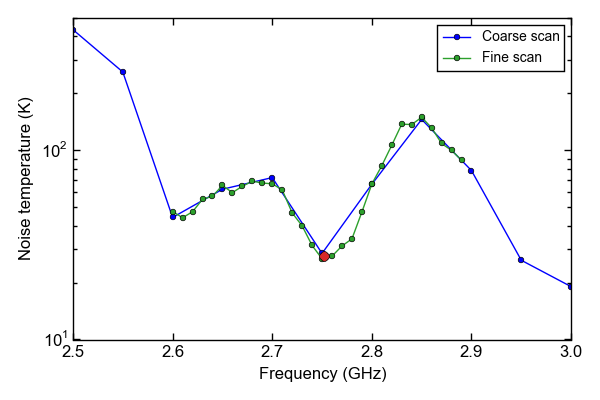
\includegraphics[width = .6\linewidth]{Figures/noise_temperature_versus_power_detailed.png}
    \caption{Detailed scan of noise temperature versus frequency in the range \SIrange{2.6}{2.9}{\giga \hertz}. The resonator with $f_0 = $\SI{2.75}{\giga \hertz} (red dot) seems to reside at a local minimum of the noise temperature.}
    \label{fig:noise temperature 2GHz}
\end{figure}

From Figure~\ref{fig:Noise temperature} it can be seen that the noise temperature can vary by a large amount between consecutive points. To determine whether this variation is due to a large uncertainty, or due to the noise temperature actually fluctuating strongly with varying frequency, a more detailed scan has been performed in the frequency region \SIrange{2.6}{2.9}{\giga \hertz}, in which one resonator has a resonance frequency. The result is shown in Figure~\ref{fig:noise temperature 2GHz}. As the curve of the detailed scan follows the curve of the coarse scan pretty closely, it can be concluded that the noise temperature of the system in fact fluctuates quite strongly with varying frequency.

Another point of interest is that the resonance frequency of the resonator lies near the local minimum of the noise temperature in that region. This is quite a stroke of luck, as a slightly higher or lower frequency would have resulted in a much higher noise temperature.



\section{Conclusion and future work}

The noise temperature gives us an estimate of the noise added to the system. It has been shown that the noise temperature can fluctuate strongly with varying frequency. In the model used to estimate the noise temperature it has been shown that outside the bandwidth of the amplifier the model breaks down. At this point the noise added by the components after the amplification, and indeed even the amplifiers themselves, needs to be taken into account to obtain accurate estimates of the noise temperature.

However, even outside of the bandwidth of the amplifier, there are frequency regions in which the noise temperature may still be acceptable. It is therefore a good idea to initially perform measurements of the noise temperature of the set-up. This will give an indication of the signal-to-noise ratio, from which accurate estimates can be made as to what the integration times for measurements should be.

The noise temperature measurements were performed using the Rhode \& Schwarz ZVM vector network analyzer. It would be interesting to see how other measurement set-ups would compare to the vector network analyzer. One interesting candidate would be a heterodyne detector. However, as the vector network analyzer can also measure phase, a fair comparison would also require the heterodyne detector to be able to measure the phase. This heterodyne detector is currently being set up, and will hopefully soon yield interesting results.

Aside from only comparing the noise temperature, other properties are also important when comparing two set-ups. One of these is the duty cycle, which is the percentage of time acually spent measuring. For the vector network analyser the duty cycle seems to be around $50\%$, provided that a single measurement sweep takes at least a few seconds. Other set-ups may therefore offer an improvement in the duty cycle. Furthermore, properties such as phase stability and uncertainty would also be interesting to compare.

Another interesting measurement would be to see if the noise temperature as a function of frequency remains the same in future cooldowns, and for different samples.


\bibliographystyle{plain}
\bibliography{bibliography}

\end{document}
